%===============================================================
\chapter{Realizando consultas con Kalcas Query Language}
 \label{cha:KQL}
%===============================================================

Como complemento a nuestra propuesta, definimos Kalcas Query Language (KQL), un DSL gr\'afico que permite realizar consultas sobre un modelo Tartarus utilizando la trazabilidad inferida y confirmada en el Cap\'itulo \ref{cha:solution}. KQL esta compuesto por dos metamodelos, uno para expresar consultas (KQLQuery) y otro que permite consignar la respuesta (KQLResponse). El modelo de consulta (conforme con KQLQuery) se entreteje con un modelo de EA (conforme con Tartarus) para obtener el modelo de respuesta (conforme con KQLResponse) aplicado a una EA particular. La respuesta al usuario se presenta como un grafo interpretado con la herramienta Graphviz, para lo cual se aplica una transformaci\'on del modelo KQLResponse a \texttt{dot}. La Figura \ref{fig:KQLTransform} describe como se transforman los diferentes modelos descritos para generar la respuesta a una consulta KQL. A continuaci\'on, vamos a describir con mayor detalle cada unos de los elementos involucrados.

%........................................................
\begin{figure} [!t]
\begin{center}
	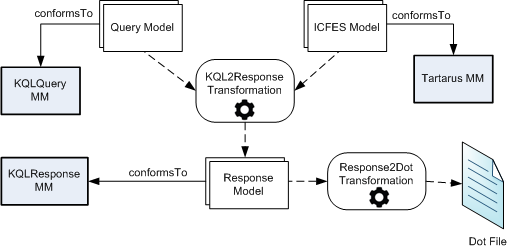
\includegraphics[scale=0.8,natwidth=507, natheight=248]{KQLTransform.png}
	\caption{Cadena de Transformaciones de Kalcas Query Language}
	\label{fig:KQLTransform}
\end{center}	
\end{figure}
%........................................................


%===============================================================
\section{Metamodelo KQLQuery}
%===============================================================

KQLQuery nos permite realizar consultas de alineaci\'on o redundancia sobre una determinada EA (modelo Tartarus), por ejemplo expresar las heur\'isticas introducidas en el Cap\'itulo \ref{cha:intro}. El metamodelo KQLQuery define los diferentes constructos del lenguaje que se pueden observar en la Figura \ref{fig:KQL_mm}. El elemento \texttt{Query} contiene las entradas de la consulta. Estas entradas pueden ser procesos y actividades en el dominio de negocio o esquemas y entidades en el dominio de informaci\'on. A partir de este metamodelo y utilizado la herramienta EuGENia \cite{Eugenia:2012} se genera un editor GMF (Graphical Modeling Framework) que permite expresar gr\'aficamente consultas en lenguaje KQLQuery. En la Figura \ref{fig:KQL_els} se puede ver el Editor KQL generado junto con los elementos que permiten dise\~nar las consultas.

%........................................................
\begin{figure} [!t]
\begin{center}
	\includegraphics[scale=0.47,natwidth=839, natheight=427pt]{KQL_mm.png}
	\caption{Metamodelo KQLQuery}
	\label{fig:KQL_mm}
\end{center}	
\end{figure}
%........................................................

%........................................................
\begin{figure} [!t]
\begin{center}
	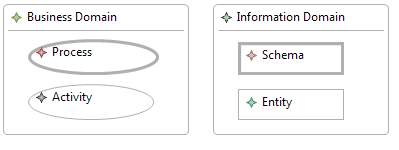
\includegraphics[scale=0.8, natwidth=399, natheight=150pt]{KQL_Elements.png}
	\caption{Elementos en el Editor KQL}
	\label{fig:KQL_els}
\end{center}	
\end{figure}
%........................................................

%........................................................
\begin{figure} [!t]
\begin{center}
	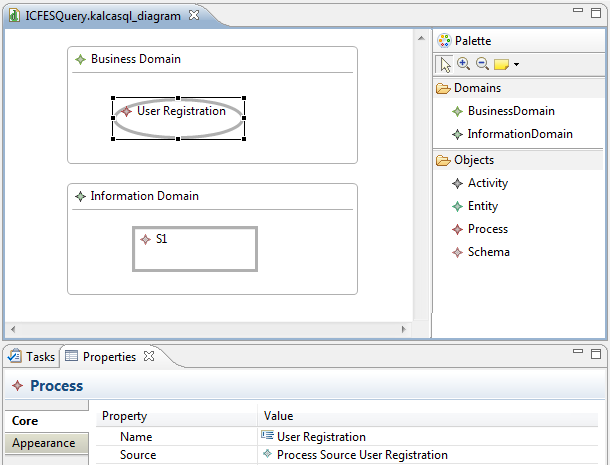
\includegraphics[scale=0.6,natwidth=610, natheight=465pt]{KQL_Question.png}
	\caption{Consulta de Alineamiento sobre el Editor KQL}
	\label{fig:KQL}
\end{center}	
\end{figure}
%........................................................


La gram\'atica KQLQuery comprende: Las secciones de dominio (Business - Information) ubicadas en la \textit{Zona de Trabajo} y los elementos de entrada en la \textit{Zona de Paleta}. Los elementos se arrastran desde la Paleta hasta las secciones de cada dominio para dise\~nar la consulta: \texttt{Process}, \texttt{Activity} (BA), \texttt{Schema} y \texttt{Entity} (IA). Estos componentes permiten definir la preguntas al modelo en t\'erminos de Negocio e Informaci\'on en diferente nivel de granularidad. Adem\'as, al definir la consulta, cada elemento puede tomar un valor no determinado \texttt{empty} (cualquier \texttt{Activity} o cualquier \texttt{Entity}) o un valor concreto del modelo (\texttt{Activity:Generar Citaci\'on} o \texttt{Entity:Citacion}). Unas vistas del editor generado se ofrecen en la Figuras \ref{fig:KQL} y \ref{fig:KQL_red}.

%........................................................
\begin{figure} [!t]
\begin{center}
	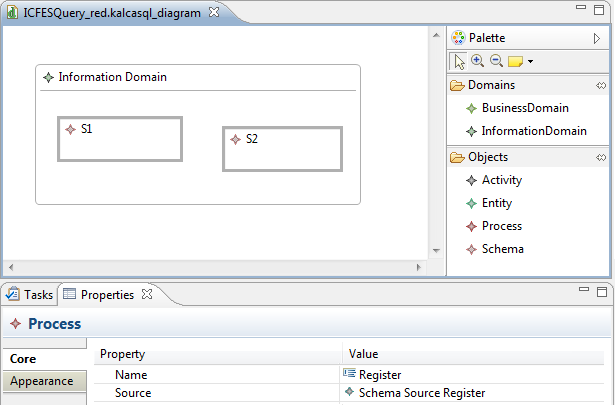
\includegraphics[scale=0.6,natwidth=612, natheight=405pt]{Redundancy_query.png}
	\caption{Consulta de Redundancia sobre el Editor KQL}
	\label{fig:KQL_red}
\end{center}	
\end{figure}
%........................................................

En la Figura \ref{fig:KQL} podemos observar una consulta de alineaci\'on (\texttt{ICFESQuery}) dise\~nada sobre nuestro caso de estudio. Se incluyen el proceso \texttt{User Registration} (Business Domain) y el Esquema \texttt{S1} (Information Domain) con el objetivo de conocer como est\'an alineados. Por otro lado, se puede ejecutar consultas de redundancias. Para este fin el usuario debe ubicar en la Secci\'on respectiva, los elementos de la paleta que desea analizar, por ejemplo en la Figura \ref{fig:KQL_red} se comparan los esquemas \texttt{Schema:S1} y \texttt{Schema:S2} en busca de redundancias. El editor gr\'afico al final construye un modelo KQLQuery que representa la pregunta que el arquitecto quiere hacer sobre el modelo Tartarus.

\section{Metamodelo KQLResponse}

El metamodelo KQLResponse presentado en la Figura \ref{fig:KQLResponse_mm} contiene los elementos resultantes de la intersecci\'on entre un modelo de consulta KQL y el modelo Tartarus. La consulta KQL se puede entender como una \textit{vista} sobre el modelo Tartatus que solo incluye los elementos involucrados y enriquecida con los conceptos de trazabilidad y redundancia. Al ser una vista parcial sobre Tartarus, el metamodelo KQLResponse tiene una estructura simplificada del metamodelo Tartarus. Encontramos las clases \texttt{InformationDomain} y \texttt{BusinessDomain}, los cuales contienen clases de tipo \texttt{Process} y/o \texttt{Schema}, mas las relaciones de redundancia (\texttt{AttrMatch} y \texttt{ProcessMatch}) o de trazabilidad (\texttt{BIAlignment}). 

Adicionalmente, como este metamodelo tiene tambi\'en prop\'ositos de an\'alisis gr\'afico, los conceptos \texttt{Entity} y \texttt{ProcessElement} poseen un atributo \texttt{aligntype} que determina, seg\'un la consulta, si el componente est\'a desalineado (\texttt{Misaligned}), alineado con un componente no incluido en la consulta (\texttt{OmittedAligned}), o alineado con un componente presente en la consulta (\texttt{Aligned}). Estas caracter\'isticas son representadas gr\'aficamente al usuario.

%........................................................
\begin{figure} [!t]
\begin{center}
	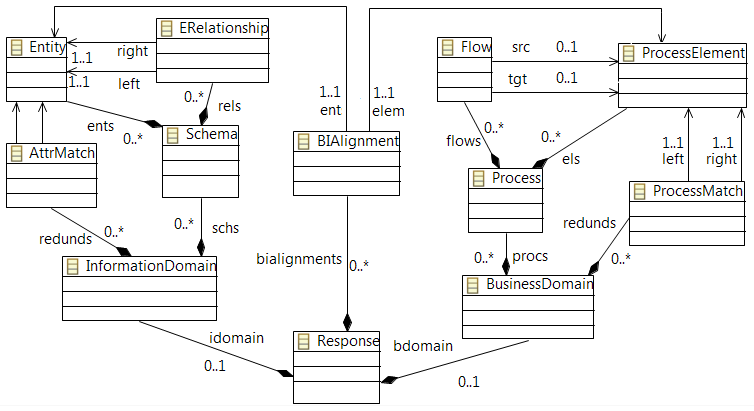
\includegraphics[scale=0.55,natwidth=754, natheight=411pt]{KQLResponse_mm.png}
	\caption{Metamodelo KQLResponse}
	\label{fig:KQLResponse_mm}
\end{center}	
\end{figure}
%........................................................

\section{Transformaci\'on Query2Response}

Para generar el modelo de respuesta conforme KQLResponse, se desarroll\'o una transformaci\'on ATL \cite{Jouault:2008} que toma de entrada los modelos KQLQuery y Tartarus para navegarlos y entretejerlos generando un modelo de salida. La transformaci\'on recorre los \texttt{Input} del modelo KQLQuery y va buscando los elementos asociados en el modelo Tartarus, con el fin de incluir todos los componentes relacionados con el elemento \texttt{Input}. 

Adicionalmente, a los objetos de clase \texttt{Activity} y \texttt{Entity} se les asigna el tipo de alineamiento (\texttt{aligntype}) de acuerdo a las alineaciones presentes en el modelo Tartarus y los criterios ingresados en el modelo de consulta. Continuando con nuestro caso de estudio, al procesar la consulta expresada en la Figura \ref{fig:KQL}, la transformaci\'on extrae todos los elementos asociados al \texttt{Proceso de Registro}, al esquema \texttt{Registro} y las relaciones \texttt{BIAlignment} contenidas dentro del modelo \texttt{ICFES.tartarus} para generar un modelo de respuesta \texttt{ResponseICFES}.

\section{Transformaci\'on Response2Dot}

Una vez obtenido el modelo de respuesta, una transformaci\'on modelo a texto es implementada con una plantilla Xpand la cual genera un archivo \textit{dot} que contiene una representaci\'on gr\'afica del modelo de respuesta. \textit{dot} permite dibujar grafos leyendo archivos de texto y produciendo archivos gr\'aficos \cite{Koutsofios:2002}. 

Los dominios de Negocio e Informaci\'on consignados en modelo KQLResponse se transforman a Cluster dentro del archivo dot. Similarmente los procesos y esquemas tambi\'en se convierten en subclusters contenidos dentro de los cluster principales (BusinessDomain o InformationDomain). Por otro lado, los ProcessElement ( i.e. \texttt{Activity, Gateway, Event}) y Entity se traducen en nodos con colores que representan su tipo de alineamiento (i.e. \texttt{Aligned=green, OmittedAligned=yellow, Misaligned=red}). Las relaciones inferidas (trazabilidad o redundancia) se representan con l\'ineas punteadas y las relaciones que ya vienen dadas desde los modelos importados (BPMN y ER) se dibujan con l\'ineas continuas. 

\begin{lstlisting}[caption={Segment of output dot file},label=lst:dot, basicstyle=\small, tabsize=2,morekeywords={digraph, subgraph, -> }]
digraph G{
subgraph cluster0 {
	label = "Business Domain";
subgraph cluster_User_Registration {
	label = "User Registration";
	Generate_Citation
	[label="Generate\nCitation", shape=box, 
	style="filled,rounded", color=green];
...
}
}
subgraph cluster1 {
	label = "Information Domain";
subgraph cluster_S1 {
		label = "S1";
		Citation [label="Citation", 
		shape=box, style="filled", color=green ];
...
}
}		
	Citation -> 
	User_Registration[style=dashed];
}	
\end{lstlisting}

\begin{landscape}
 
%........................................................
\begin{figure} 
\begin{center}
	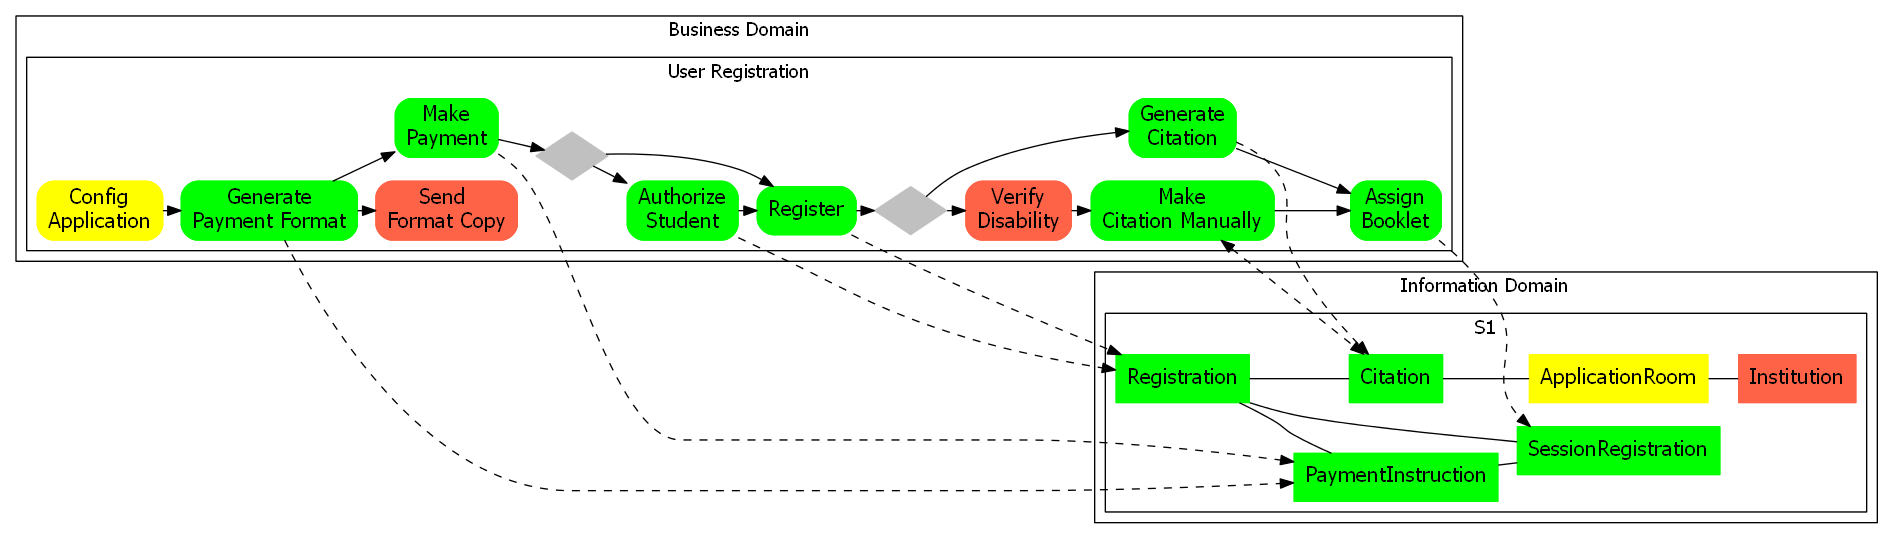
\includegraphics[scale=0.3,natwidth=1893, natheight=539pt]{align.png}
	\caption{Salida de una Consulta de Alineamiento en KQL}
	\label{fig:KQL_out}
\end{center}	
\end{figure}
%........................................................

%........................................................
\begin{figure} [!t]
\begin{center}
	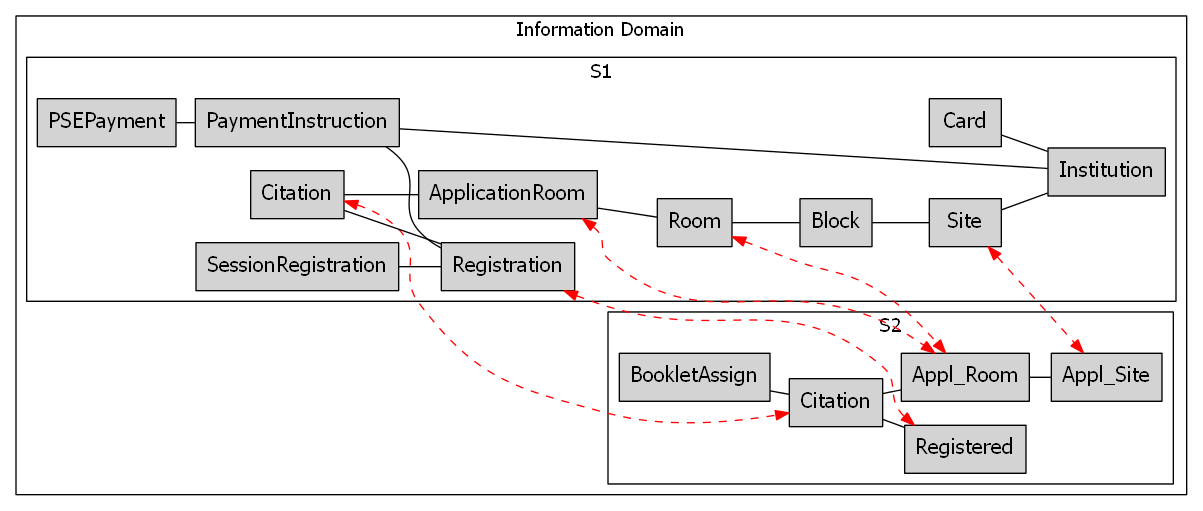
\includegraphics[scale=0.3,natwidth=1349, natheight=591pt]{redund.png}
	\caption{Salida de una Consulta de Redundancia en KQL}
	\label{fig:KQL_out2}
\end{center}	
\end{figure}
%........................................................

\end{landscape}

El Listado \ref{lst:dot} es un segmento del archivo dot de salida donde se puede apreciar la estructura jer\'arquica de clusters, as\'i como los componentes de cada dominio enriquecidos con elementos gr\'aficos. Este archivo dot es interpretado por Graphviz y genera la imagen que se presenta en la Figura \ref{fig:KQL_out}. La imagen corresponde a la consulta expresada en previamente en la Figura \ref{fig:KQL}. Este reporte permite identificar los procesos que no tienen trazabilidad en el dominio de informaci\'on y viceversa. Otro ejemplo es la salida de la consulta de redundancia dise\~nada en la Figura \ref{fig:KQL_red} que se presenta en la Figura \ref{fig:KQL_out2}.

Tanto los objetos que aparecen \texttt{Misaligned} al ejecutar una \texttt{Alignment Query} (i.e. actividad \texttt{Send Format Copy} y entidad \texttt{Institucion}) como los objetos incluidos en el resultado de una \textit{Redundancy Query} (i.e. Entidades Citation) constituyen los potenciales desalineamientos evaluados por las heur\'isticas referidas en el Cap\'itulo \ref{cha:intro}.